\documentclass[graphics]{beamer}

\usepackage{graphicx}
\usepackage{verbatim}
\usepackage{wrapfig}
\useoutertheme{shadow}
%\usecolortheme{orchid}
\usecolortheme{seahorse}


% math commands
\newcommand{\be}{\begin{eqnarray}}
\newcommand{\ee}{\end{eqnarray}}
\newcommand{\beq}{\begin{equation}}
\newcommand{\eeq}{\end{equation}}
\def\simless{\mathbin{\lower 3pt\hbox
      {$\rlap{\raise 5pt\hbox{$\char'074$}}\mathchar"7218$}}}
\def\simgreat{\mathbin{\lower 3pt\hbox
      {$\rlap{\raise 5pt\hbox{$\char'076$}}\mathchar"7218$}}} %> or of order

% variables

\def\toonscale{0.45}
\def\mboxy#1{\mbox{\small #1}}


\begin{comment}
\AtBeginSection[]{
  \frame{
    \frametitle{Outline}
    \tableofcontents[currentsection]
  }
}
\end{comment}

\title{Neutrino Torques
}
\subtitle{}
\author[U. Pen]{\textcolor{green}{Ue-Li Pen, Haoran Yu, Xin Wang}
\\[8mm] 
}
\date{October 26, 2018}


\begin{document}

\frame{
\begin{picture}(320,250)
\put(-50,-130){
\includegraphics[width=5.5in]{Figures/delta_nu_sim.pdf}}
\end{picture}
\vspace{-3in}
\titlepage
}

%\section*{Introduction}
\section{Cosmological Neutrino Clustering}

\begin{comment}
  \subsection{Outline}

  \frame{
    \frametitle{Outline}
    \tableofcontents
  }
\end{comment}

  \frame{
\vspace{-0.5in}
    \frametitle{Neutrinos}
    \begin{itemize}     
    \item defy expectations: existence, mass, oscillation, large
      mixing angles -- fruitful discvery space
        \item minimum mass 0.06 eV: $\Omega_\nu \sim 10^{-3} \ll \Omega_b$
        \item most massive neutrino non-relativistic today, affects LSS
        \item normal or inverted hierarchy?
        \item cosmological probes: how to disentangle such a small
          effect
        \item statistics not main problem: SDSS $1/\sqrt{n} \sim
          10^{-3}$
        \item arXiv:1810.11784
%          \vspace{-0.15in}
    \end{itemize}
  }
  \frame{
    \frametitle{Observables}
    \begin{itemize}
        \item CMB, gravitational lensing: 2-D projection, 
        \item galaxies: 3-D biased displacement field
        \item Monge-Amp\'ere equation/solution
        \item ideally measure 2 fields, infer 2 fields: CDM, neutrinos (HDM)
    \end{itemize}
\vspace{-0.1in}\hspace{.3in}
\includegraphics[width=2.2in]{Figures/th2photo.jpg}
}
  \frame{
    \frametitle{Movie}
    {\tt http://cita.utoronto.ca/\~\,haoran/thnu/movie.html}
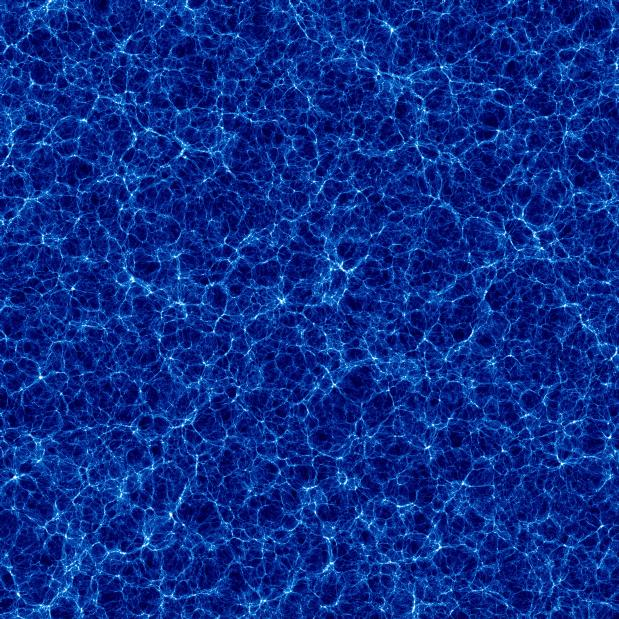
\includegraphics[width=4.2in]{Figures/thnucdmlowres.jpg}
}
  \frame{
    \frametitle{Galaxy Spins}
    \begin{itemize}
        \item most galaxies are rotating disks of stars and gas
        \item readily identifyable spin axis
        \item dust lanes, trailing spiral arms, HI velocity (rotation) field
     \end{itemize}
}
\frame{
    \frametitle{Observable}
\includegraphics[width=4.1in]{Figures/M51s.jpg}  

(M51, from Wikipedia)
  }

  \frame{
    \frametitle{Angular momentum}
    \begin{itemize}
        \item 1st order effect from misalignment of moment of inertia
          and tidal tensor
        \item $\tau\equiv\int \rho \bf{r} \times \nabla \phi$
        \item $\tau_i=\epsilon_{ijk} \int \rho x^jx^l \partial_l\partial_k\phi \equiv\epsilon_{ijk} I_{il}T_{lk}$
        \item $\tau= * I \cdot T$
        \item first realized by S. White (1984), see also LP00
     \end{itemize}
}


\frame{
    \frametitle{3-D: E-mode}
%\vspace{-0.5in}
\hspace{-0.2in}\includegraphics[width=2.3in]{Figures/nonlinear.png}  
\vspace{0.15in}\includegraphics[width=2.21in]{Figures/reconstructed.png}  

Eulerian (L) vs Lagrangian (R) (from Yu et al 2016, 1610.7112)
  }

\frame{
    \frametitle{Lagrangian coordinates}
\center{\includegraphics[width=4.3in]{Figures/delta_reco_raw.pdf}  }
  }

  \frame{
    \frametitle{Coordinate freedom}
\begin{eqnarray}
{\rm potential\ deformation\ \ \ \ \ }  x^i &=& \xi^\mu \delta^i_\mu + \frac{\partial \phi}{\partial
    \xi^\mu}\delta^{i\mu}\nonumber\\
{\rm dreibein\ \ \ \ \ \  } e^i_\mu &\equiv& \partial x^i / \partial \xi ^ \mu \nonumber\\
 {\rm volume\  element\ \ \ \ }\sqrt{g} &\equiv& \mathrm{det}\left| e^i_\mu\right|\nonumber\\
{\rm mass\ coordinate \ \ \ \ \ }    \rho \sqrt{g}&=&\mathrm{Const.}\nonumber\\
    \partial _\mu (\rho \sqrt{g} e^\mu _i \delta^{i\nu}
    \partial_\nu \dot{\phi})&=&\langle\rho\rangle-\rho \sqrt{g}
\label{eqn:dif}
\end{eqnarray}
Solve Monge-Amp\'ere eqn (\ref{eqn:dif}) using multigrid (Pen 1995):
unique bijective mass coordinate.  See also Tully/Peebles, Mohayaee+, Goldberg, Schmidtfull, Wang+, Seljak,
Zaldarriaga, Hada/Eisenstein, Shi/Brikin/Li+, Jasche+, Sarpa+
}

  \frame{
    \frametitle{Multigrid solution}
\vspace{-0.7in}\center{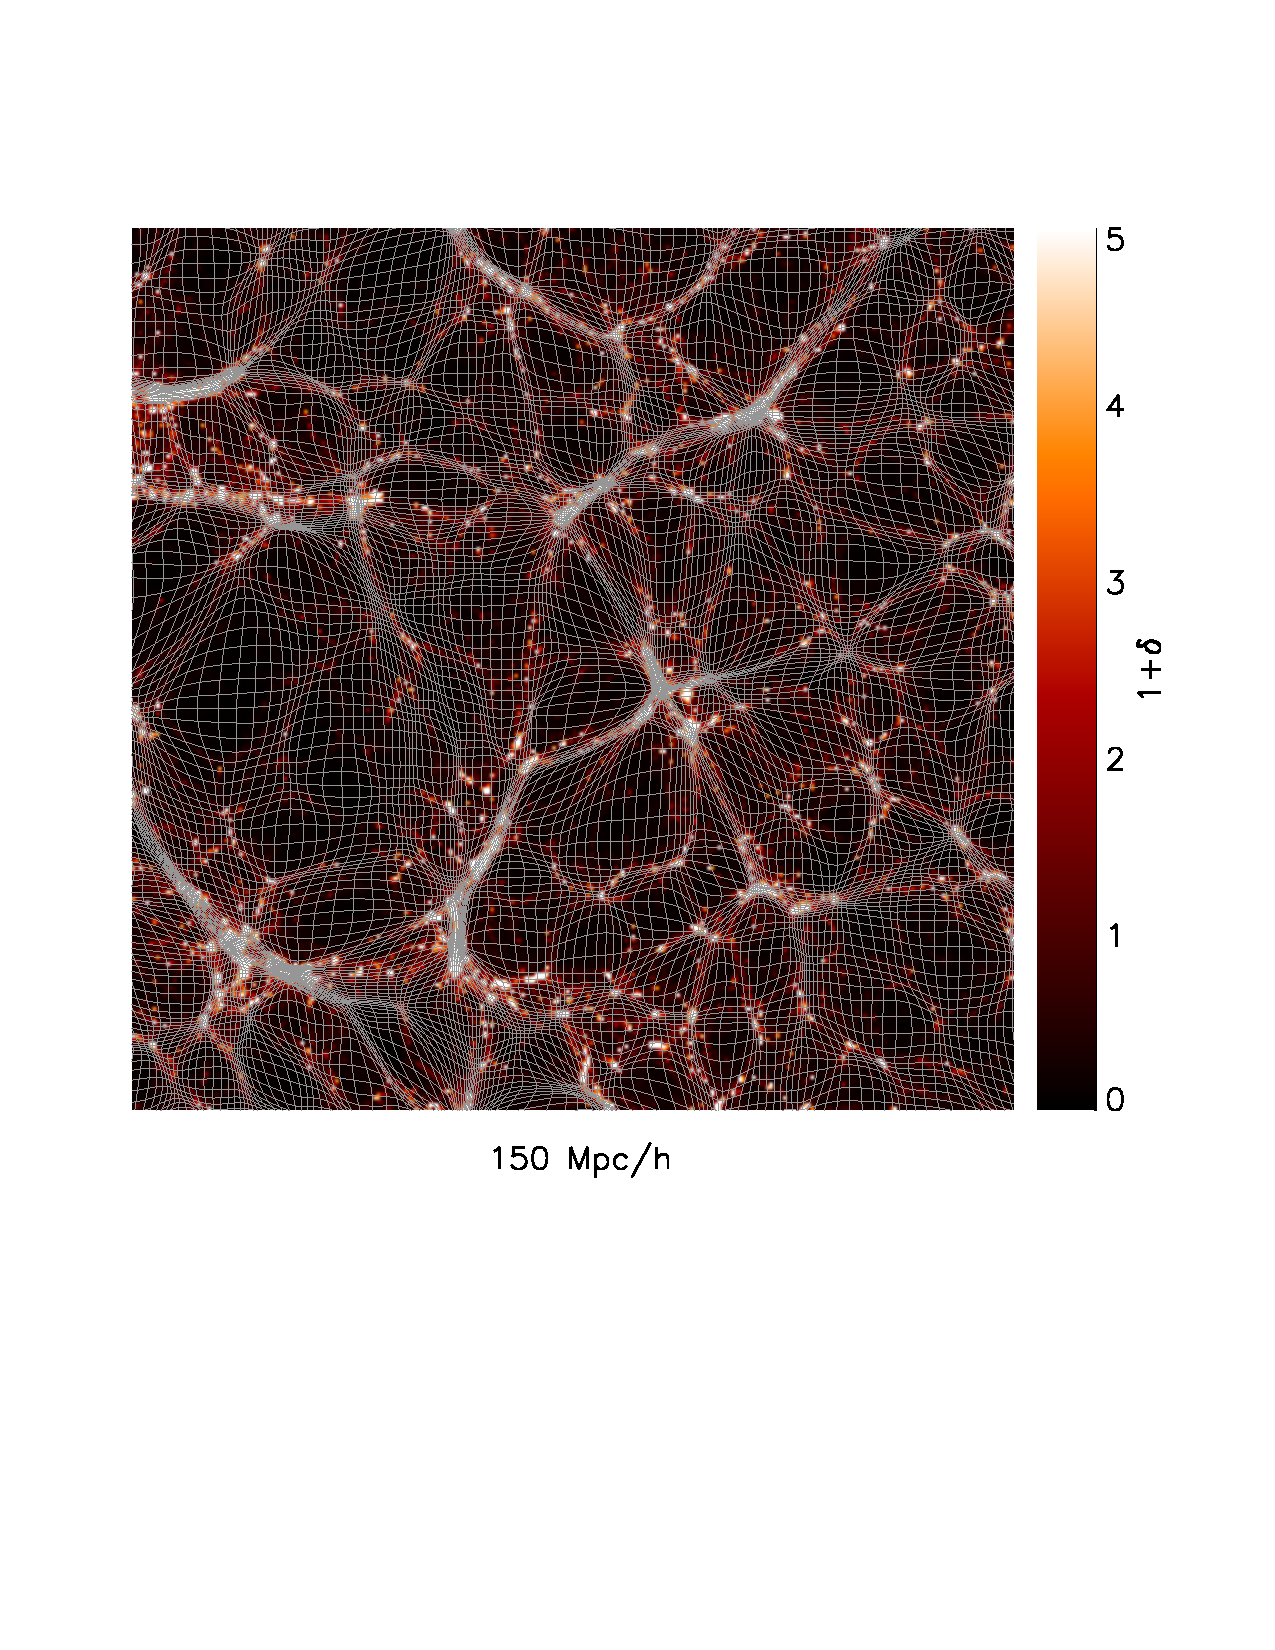
\includegraphics[width=4.0in]{Figures/map0512-0128_i1500_xz222.pdf}}
Zhu et al 1610.09638
}
  \frame{
    \frametitle{Redshift space}
\vspace{-0.7in}\center{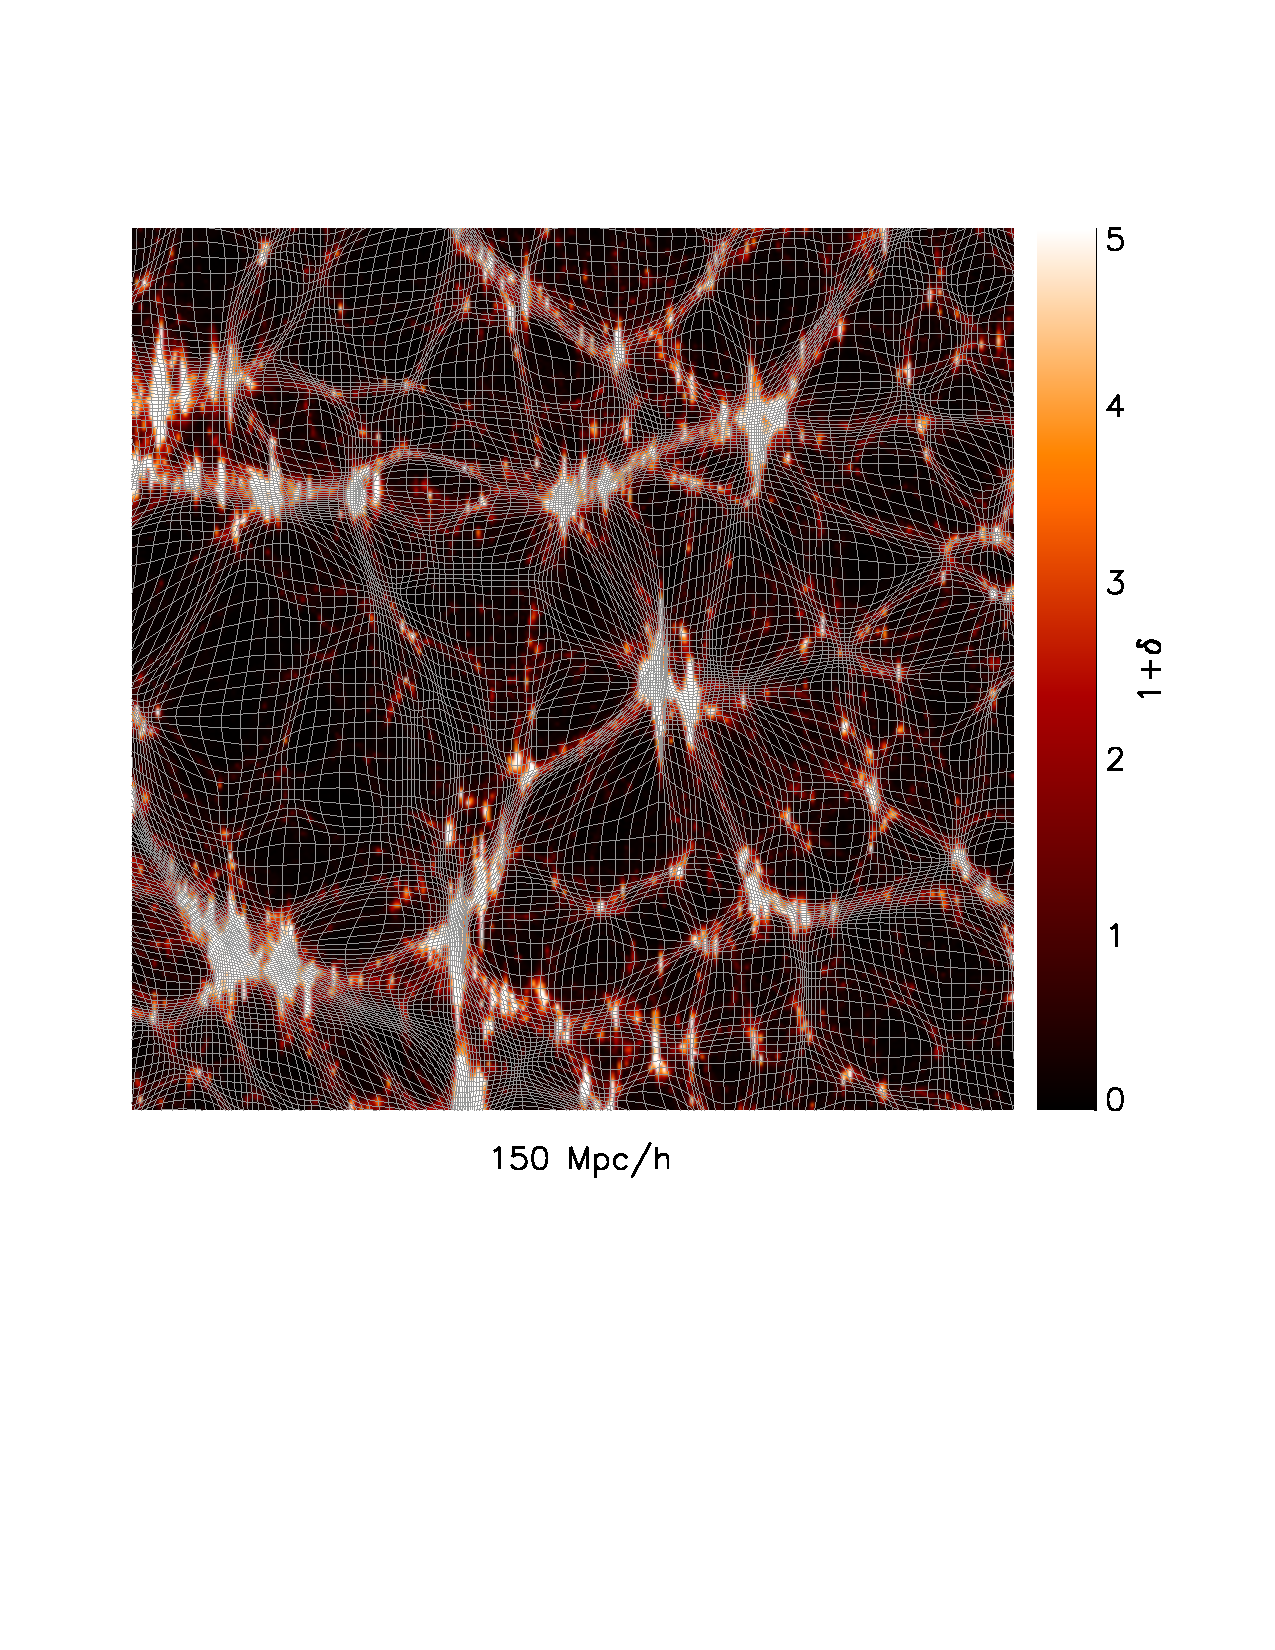
\includegraphics[width=4.0in]{Figures/map0512-0128_i0900_xz222_rsd3.pdf}}
Zhu et al 1610.09638
}

  \frame{
    \frametitle{Low noise limit}
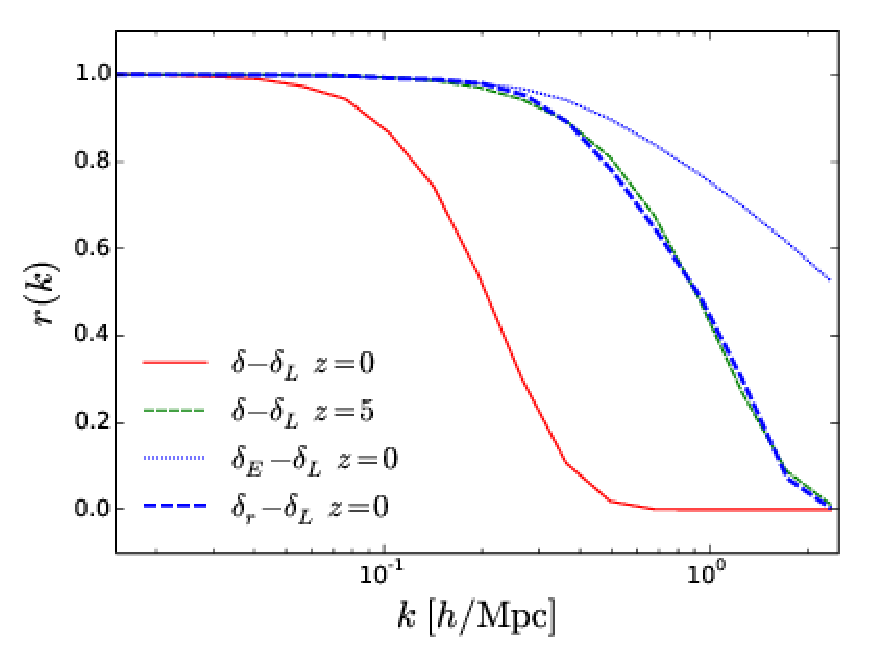
\includegraphics[width=3.4in]{Figures/rk.pdf}
}
  \frame{
    \frametitle{Halos}
\vspace{-0.5in}\hspace{-0.9in}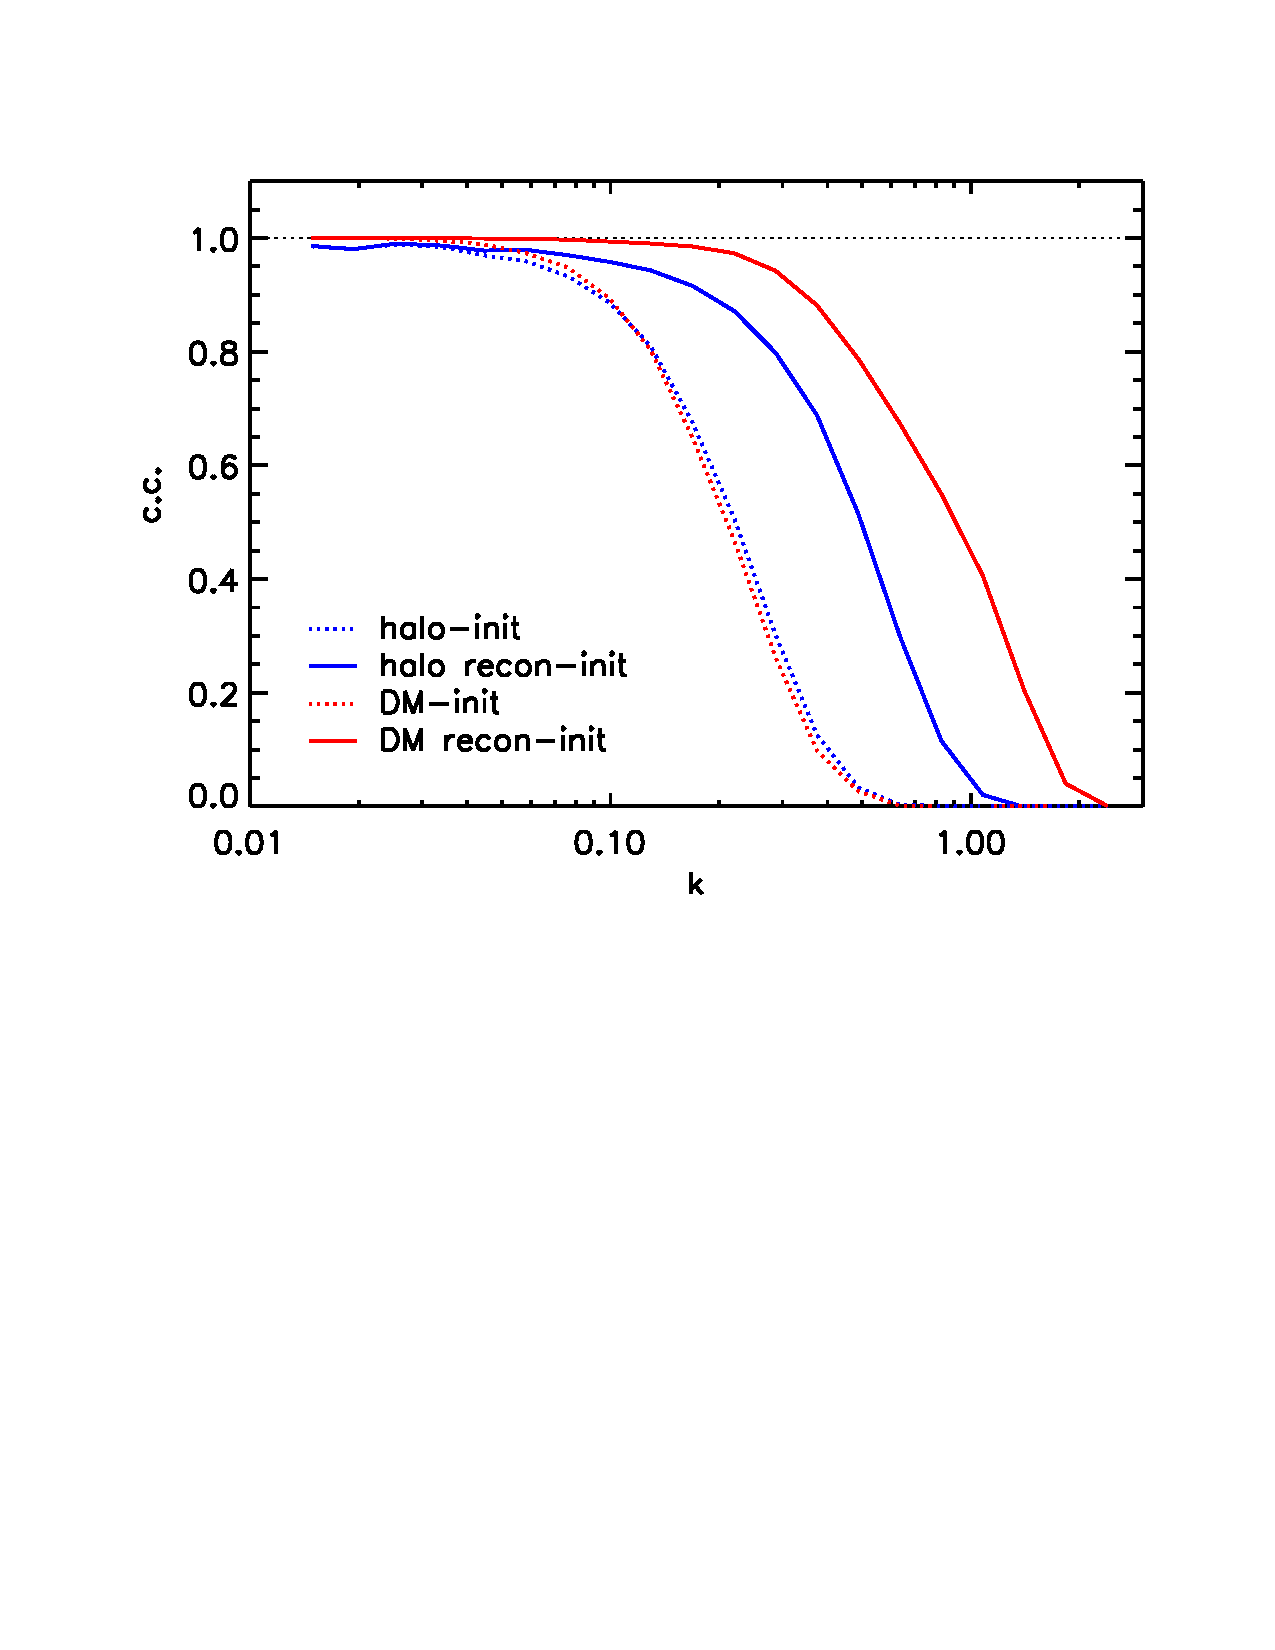
\includegraphics[width=5.0in]{Figures/halocc.pdf}
}

 \frame{
    \frametitle{Predicting Neutrino Torques}
    \begin{itemize}
      \item $\Delta x (q) = q^j \partial_i\partial_j \psi$
        \item $I_c \sim T_c$: both describe particle displacement
        \item $j_\nu = \epsilon T_c T_\nu$
        \item Neutrino tidal torque is predictable observable from
          displacement potential
     \end{itemize}
  }
  \frame{
    \frametitle{Illustration}
\vspace{-0.5in}\hspace{-0.6in}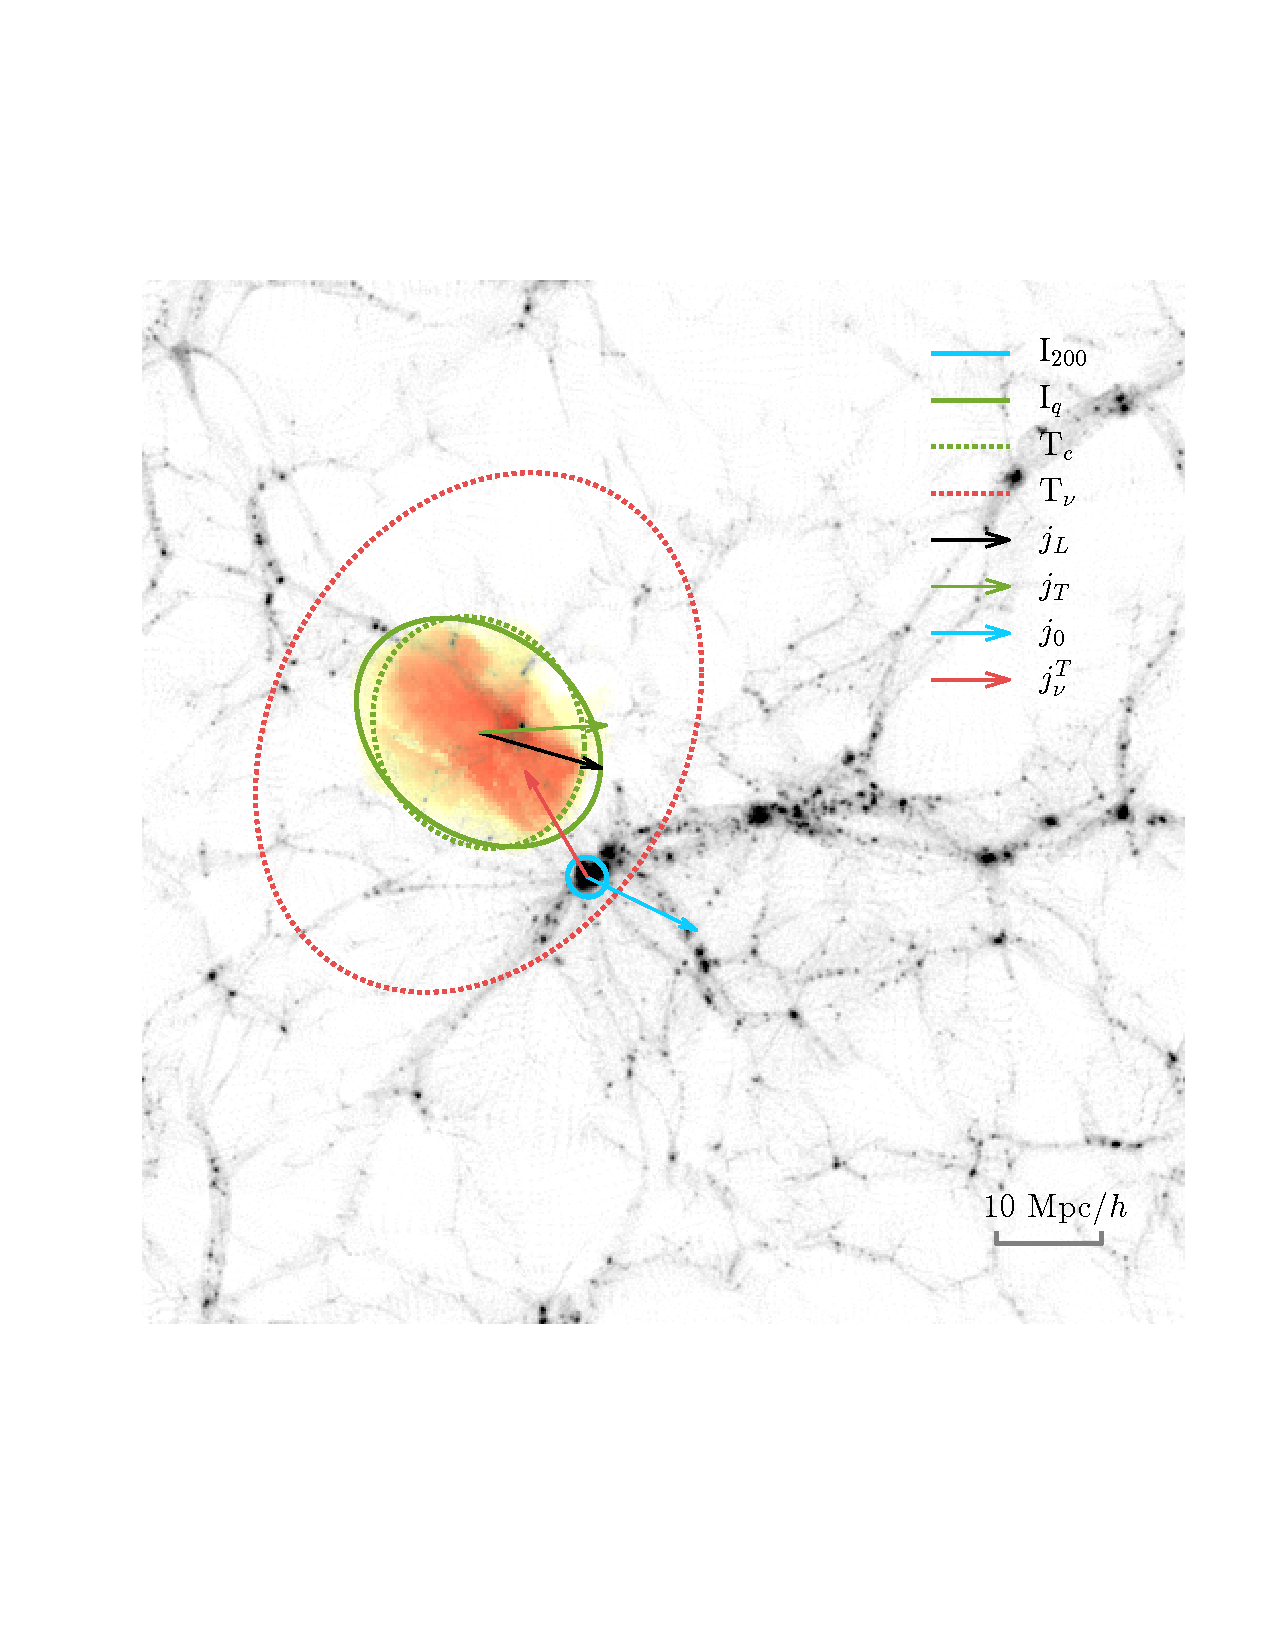
\includegraphics[width=5.0in]{Figures/f1.pdf}
}

 \frame{
    \frametitle{Size estimate}
    \begin{itemize}
    \item $|j_\nu/j_c| \sim 10^{-4} (f_\nu /0.003) (\sqrt{P(k_{\rm FS})/P(k_{\rm vir})}/0.03$
    \item agrees with simulation measurement
    \item need $n> 10^8$ galaxy spins
    \item accessible in next generation 21cm surveys
     \end{itemize}
  }


  \frame{
\vspace{-0.5in}
    \frametitle{Future 21cm Surveys}
    \begin{itemize}
        \item expand on HSHS (Peterson et al 2006), CHIME
        \item build on economy of scale, map $10^{11}$ galaxies
     \end{itemize}
  }
  
\frame{
\vspace{-0.5in}
    \frametitle{More cosmological applications}
    \begin{itemize}
        \item map initial (linear) tidal field
        \item BAO, standard ruler (Alcock-Paczynski effect)
        \item modified gravity, time evolving neutrino mass
     \end{itemize}
  }


\frame{
\vspace{-0.5in}
    \frametitle{Conclusions}
    \begin{itemize}
      \item galaxy spins: new probe of initial conditions
      \item predictable from observable displacement field using
        non-linear reconstruction
      \item computationally straightforward, mass coordinate
            similar to Lagrangian
          \item already observable, scalable to much larger surveys
          \item parity odd field, less likely to be contaminated
          \item enables measurement of 2 cosmic scalar fields:
            potential beat cosmic variance limits, etc
     \end{itemize}
  }


\end{document}
